% Slides for 2024-09-30
\begin{frame}{Dual Laser}
    \centering
    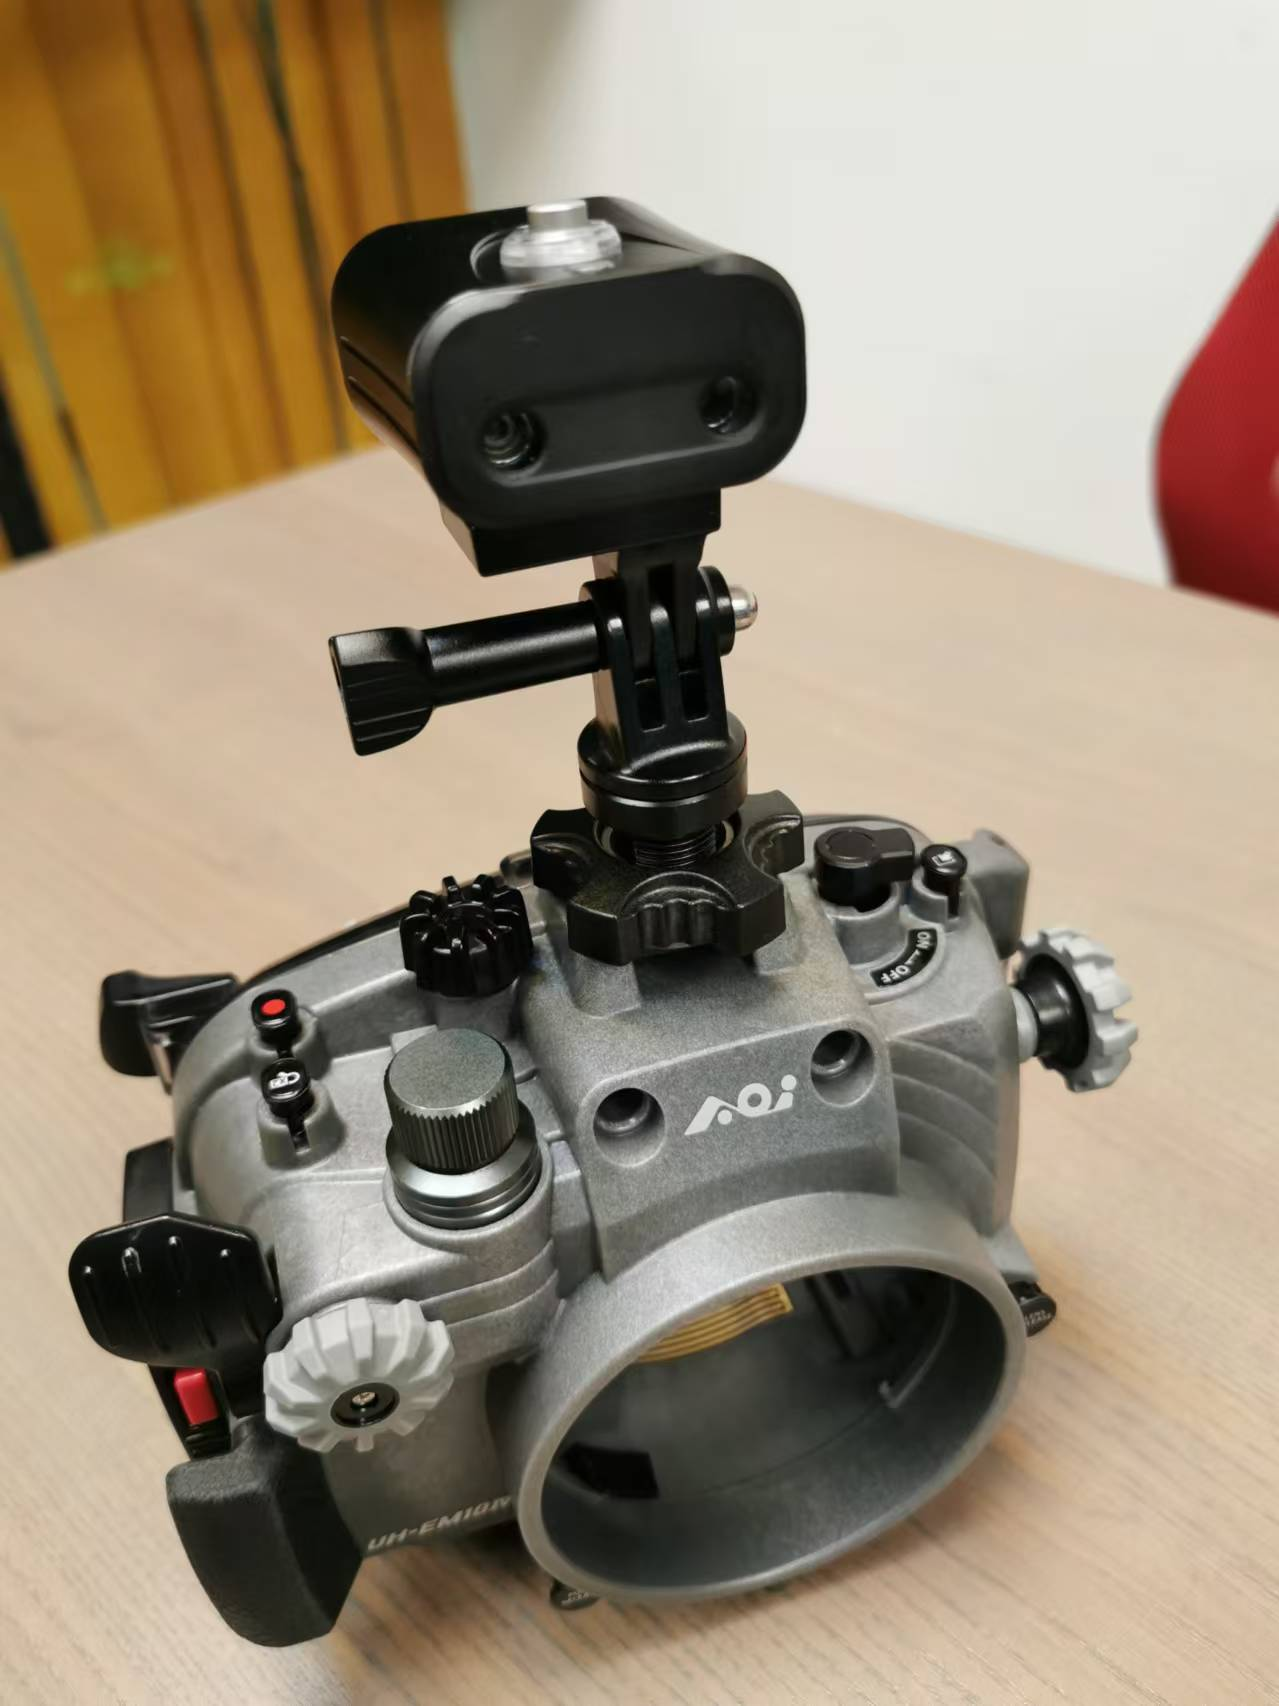
\includegraphics[height=0.7\textheight,width=0.7\textwidth,keepaspectratio]{images/fs_duallaser.jpg}
\end{frame}

\begin{frame}{Weekly Diving}
    \centering
    \includegraphics[height=0.7\textheight,width=0.7\textwidth,keepaspectratio]{images/fs_dive.jpg}
\end{frame}

\begin{frame}{Post Summer Work}
    \begin{itemize}
        \item Additional fishsense-lite CLI work - can process data
    \end{itemize}
\end{frame}

\begin{frame}{FishSense Split}
    \begin{enumerate}
        \item Aqua3D Fundamental (KRG) - Fundamental research into underlying camera technologies
        \item Aqua3D Engineering (E4E) - Leverage the fundamental research into usable depth-of-field cameras
        \item FishSense Core Technologies (E4E) - Leverage existing "third-party" cameras for fish length measurement, including Grouper Moon
        \item FishSense End User Technologies (E4E) - User-facing applications which can measure fish
    \end{enumerate}
\end{frame}

\begin{frame}{199}
    \begin{itemize}
        \item Tongfei - Focused on Grouper Moon related projects
        \item Kyle - Focused on improving scale by building web technology
    \end{itemize}
\end{frame}

% To create a slide, use the following:
% \begin{frame}{TITLE}
%     BODY
% \end{frame}

% To create a slide with a bullet list, use the following:
% \begin{frame}{TITLE}
%     \begin{itemize}
%         \item ITEM 1
%         \item ITEM 2
%     \end{itemize}    
% \end{frame}

% To create a slide with numbered list, use the following:
% \begin{frame}{TITLE}
%     \begin{enumerate}
%         \item ITEM 1
%         \item ITEM 2
%     \end{enumerate}
% \end{frame}

% To create a slide with a graphic:
% 1. Add the graphic to this folder (named picture.png)
% 2. Use the following:
% \begin{frame}{TITLE}
%     \centering
%     \includegraphics[height=0.7\textheight,width=0.7\textwidth,keepaspectratio]{picture.png}
% \end{frame}

% To create a slide with two columns, use the following:
% \begin{frame}{TITLE}
%     \begin{columns}
%         \begin{column}{0.5\textwidth}
%             COLUMN 1 BODY
%         \end{column}
%         \begin{column}{0.5\textwidth}
%             COLUMN 2 BODY
%         \end{column}
%     \end{columns}
% \end{frame}
